\documentclass[10pt]{article}

\usepackage{amsmath,amscd}
\usepackage{amssymb,array}
\usepackage{amsfonts,latexsym}
\usepackage[mathscr]{euscript}
\usepackage{graphicx,subfig,wrapfig}
\usepackage{times}
\usepackage{psfrag,epsfig}
\usepackage{verbatim}
\usepackage{tabularx}

\newcommand{\matlab}[1]{\texttt{#1}}
\newcommand{\setname}[1]{\textsl{#1}}
\newcommand{\Ce}{\mathbb{C}}
\newcommand{\Ree}{\mathbb{R}}
\newcommand{\p}{\begin{pmatrix}}
\newcommand{\pp}{\end{pmatrix}}
\newcommand{\bm}{\begin{bmatrix}}
\newcommand{\bb}{\end{bmatrix}}
\newcommand{\eul}[1]{e^{#1}}

\begin{document}

\title{ \vspace{-30mm}Systems Bioengineering 3\\Homework 11}
\author{Greg Kiar}

\maketitle
\begin{enumerate}


%q1
\item We are given that: \begin{align*} G_T &= G + GX_n + GY_n \\ G + nX &\rightleftharpoons GX_n \\ G + nY &\rightleftharpoons GY_n \\ \end{align*}
\begin{enumerate}
\item \begin{align*} GX^n &= G X_n \\ \frac{GX_n}{G} &= X^n \end{align*}
\item \begin{align*} GY^n &= G Y_n \\ \frac{GY_n}{G} &= Y^n \end{align*}
\item \begin{align*} f &= \frac {GX_n + GY_n}{G_T} \\ &= \frac {GX_n + GY_n}{G + GX_n + GY_n} \\ &= \frac {X^nG + Y^nG}{G + X^nG + Y^nG} \\ f &= \frac{X^n + Y^n}{1 + X^n + Y^n} \end{align*}
\item The figure plotted for the previous calculations is shown below.\\ 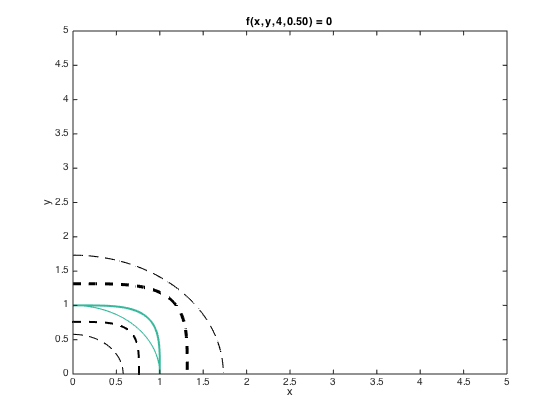
\includegraphics[scale=0.4]{hw11q1d.png}
\item I would describe the behaviour of this function in logic terms as an $OR$ gate; the logic function is $f = a + b$. Upon inspection of the graph, you can see that when either the $X$ or $Y$ term is large, they contribute to activate the function. However, when both $X$ and $Y$ are small, the function goes to zero. This, of course, is equivalent to a $NAND$ gate as well.
\end{enumerate}


%q2
\item We are given that: \begin{align*} \\ G + nX + nY &\rightleftharpoons GX_nY_n \end{align*}
\begin{enumerate}
\item \begin{align*} GX^nY^n &= G X_n Y_n \\ \frac{GX_nY_n}{G} &= X^nY^n \end{align*}
\item \begin{align*} f &= \frac {GX_nY_n}{G_T} \\ &= \frac {GX_nY_n}{G + GX_nY_n} \\ &= \frac {GX^nY^n}{G + GX^nY^n} \\ f &= \frac{X^nY^n}{1 + X^nY^n} \end{align*}
\item The figure plotted for the previous calculations is shown below.\\ 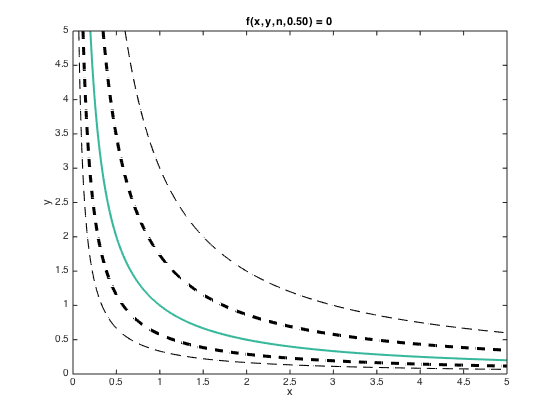
\includegraphics[scale=0.4]{hw11q2c.png}
\item I would describe the behaviour of this function in logic terms as an $AND$ gate; the logic function is $f = a \and b$. Upon inspection of the graph, you can see that only when the $X$ and $Y$ terms are large, do they contribute make the function nonzero. However, when either $X$ or $Y$ are small, the function goes to zero. This, of course, is equivalent to a $NOR$ gate as well.
\item As can be seen in the figure below, when $n$ increases, the sharpness of this relationship increases. This means that as the value of $n$ increases, the function more closely matches the $AND$ logic function. Also the $f = 0.75$ and $f=0.25$ lines approach the $f=0.5$ line more closely. \\ 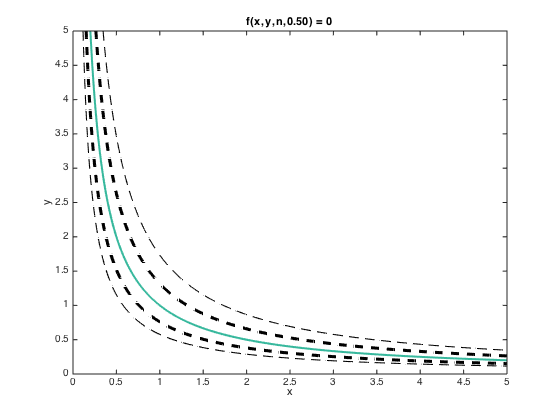
\includegraphics[scale=0.4]{hw11q2e.png}
\end{enumerate}


%q3
\item We are given that: \begin{align*} G + nX &\rightleftharpoons GX_n \\ G + nY &\rightleftharpoons GY_n \end{align*}
\begin{enumerate}
\item \begin{align*} f &= \frac {GX_n}{G_T} \\ &= \frac {GX_n}{G + GX_n+ GY_n} \\ &= \frac {GX^n}{G + GX^n+GY^n} \\ f &= \frac{X^n}{1 + X^n+Y^n} \end{align*}
\item The figure plotted for the previous calculations is shown below.\\ 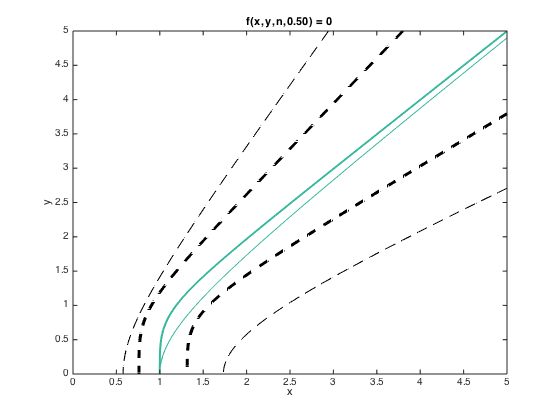
\includegraphics[scale=0.4]{hw11q3b.png}
\item I would describe the behaviour of this function in logic terms as an $AND$ gate with an inverted $a$ input;  the logic function is $f = \bar{a} \bar{b}$ where $\bar{a}$ is the inverted value of $a$. Upon inspection of the graph, you can see that only when the $Y$ term is large and the $X$ is small, does the function grow. However, when $X$ is large or $Y$ is small, the function goes to zero.
\end{enumerate}


%q4
\item We are given that: \begin{align*} G + nX &\rightleftharpoons GX_n \\ GX_n + nY &\rightleftharpoons GX_nY_n \end{align*}
\begin{enumerate}
\item \begin{align*} f &= \frac {GX_n}{G_T} \\ &= \frac {GX_n}{G + GX_n + GX_nY_n} \\ &= \frac {GX^n}{G + GX^n+GX^nY^n} \\ f &= \frac{X^n}{1 + X^n+X^nY^n} \\ \end{align*}
\item The figure plotted for the previous calculations is shown below.\\ 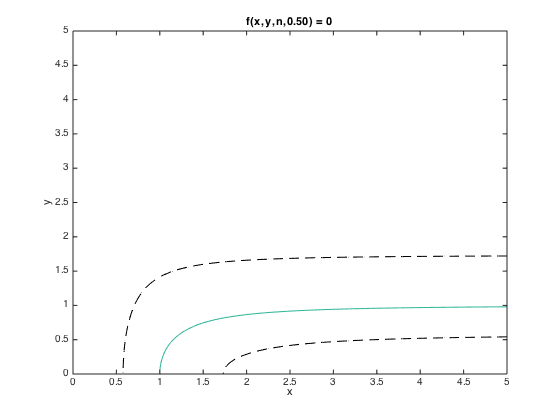
\includegraphics[scale=0.4]{hw11q4b.png}
\item I would describe the behaviour of this function in logic terms as an $OR$ gate with an inverted $a$ input;  the logic function is $f = \bar{a} + b$ where $\bar{a}$ is the inverted value of $a$. Upon inspection of the graph, you can see that only when the $X$ term is small or the $Y$ is large, does the function grow. However, when $X$ is large and $Y$ is small, the function goes to zero.
\item Comparing this trend to that obtained in the section 3 above, we can see a sharper response in this model. When a repressor is used instread of a competetive activator, we see a much more consistently controlled response.
\end{enumerate}


%q5
\item We are given that: \begin{align*}  f = \frac{X^2 + Y^2 + X^2Y^2}{1+X^2 + Y^2 + X^2Y^2 + Z^2 + X^2Y^2Z^2} \end{align*}
\begin{enumerate}
\item Based on the equation $f$ given, we can derive that the following are the transciptional complexes which can bind to this promoter: \begin{align*} GX_2 & & &GY_2 & GX_2Y_2 \\ GZ_2  &&& GX_2Y_2Z_2 \end{align*}
\item Assuming that trascriptionally active refers to having active involvement in the process of transcription, then we can isolate the transcriptional complexes that appear within the numerator of $f$ as being our transcriptionally active complexes. They are: \begin{align*} GX_2 && GY_2 && GX_2Y_2 \end{align*}
\item Given the revised formula depicting the forward rate of transcription, the coefficients $\beta_{1,2,3}$ would represent rates of the binding of each type of transcriptional complex. For instance, this could be shown as follows: \begin{align*} G + 2X &\overset{\beta_1}{\rightleftharpoons} GX_2 \\ G + 2Y &\overset{\beta_2}{\rightleftharpoons} GY_2 \\ G + 2X + 2Y &\overset{\beta_3}{\rightleftharpoons} GX_2Y_2 \end{align*}
\end{enumerate}
\end{enumerate}
\end{document}
